\documentclass[11pt]{article}

\input{../../Latex_Common/skinnerr_latex_preamble_asen5417.tex}

%%
%% DOCUMENT START
%%

\begin{document}

\pagestyle{fancyplain}
\lhead{}
\chead{}
\rhead{}
\lfoot{\hrule ASEN 5417: Homework 7}
\cfoot{\hrule \thepage}
\rfoot{\hrule Ryan Skinner}

\noindent
{\Large Homework 7}
\hfill
{\large Ryan Skinner}
\\[0.5ex]
{\large ASEN 5417: Numerical Methods}
\hfill
{\large Due 2015/12/1}\\
\hrule
\vspace{6pt}

%%%%%%%%%%%%%%%%%%%%%%%%%%%%%%%%%%%%%%%%%%%%%%%%%
%%%%%%%%%%%%%%%%%%%%%%%%%%%%%%%%%%%%%%%%%%%%%%%%%
\section{Introduction} %%%%%%%%%%%%%%%%%%%%%%%%%%
%%%%%%%%%%%%%%%%%%%%%%%%%%%%%%%%%%%%%%%%%%%%%%%%%
%%%%%%%%%%%%%%%%%%%%%%%%%%%%%%%%%%%%%%%%%%%%%%%%%

Consider the non-linear, inviscid Burgers equation for $u(x,t)$,
\begin{equation}
\pp{u}{t} + u \pp{u}{x} = 0
\;,
\end{equation}
with the initial conditions
\begin{equation}
\begin{aligned}
u(x,0) &= 10 &\quad 0  \le\; &x \le 30 \;, \\
u(x,0) &= 0  &\quad 30 \le\; &x \le 40 \;.
\end{aligned}
\end{equation}

Use the following finite-difference approximations to numerically integrate this equation using appropriate Dirichlet or Neumann BCs on an $x$-grid with $\Delta x = 0.2$:
\begin{enumerate}
\item MacCormack explicit method
\item Beam and Warming implicit method
\end{enumerate}

Note that the second method  may require the incorporation of a smoothing operator added directly to the finite difference formula. Using a fourth-order artificial viscosity, optimize the coefficient of this operator for minimum amplitude errors,
\begin{equation}
D_\epsilon = - \epsilon(\Delta x)^4 \pp{^4 u}{x^4}
\;,
\end{equation}
where the negative sign ensures that positive dissipation is produced. Using central differences, we obtain
\begin{equation}
\epsilon(\Delta x)^4 \pp{^4 u}{x^4} = u_{i-2} -4u_{i-1} +6u_i -4u_{i+1} +u_{i+2}
\;.
\end{equation}
The coefficient $\epsilon$ generally obeys $0 \le \epsilon \le 1/8$, with a preferred value of $\epsilon = 0.1$.

For both methods, plot the solutions at intervals of about two time units up to about $t=8$ time units. Obtain solutions for Courant numbers of $C = \{\tfrac{3}{4}, 1, \tfrac{5}{4}\}$. Comment on the stability of the scheme and dispersive/dissipative errors.

%%%%%%%%%%%%%%%%%%%%%%%%%%%%%%%%%%%%%%%%%%%%%%%%%
%%%%%%%%%%%%%%%%%%%%%%%%%%%%%%%%%%%%%%%%%%%%%%%%%
\section{Methodology} %%%%%%%%%%%%%%%%%%%%%%%%%%%
%%%%%%%%%%%%%%%%%%%%%%%%%%%%%%%%%%%%%%%%%%%%%%%%%
%%%%%%%%%%%%%%%%%%%%%%%%%%%%%%%%%%%%%%%%%%%%%%%%%

%%%%%%%%%%%%%%%%%%%%%%%%%%%%%%%%%%%%%%%%%%%%%%%%%
%%%%%%%%%%%%%%%%%%%%%%%%%%%%%%%%%%%%%%%%%%%%%%%%%
\section{Results} %%%%%%%%%%%%%%%%%%%%%%%%%%%%%%%
%%%%%%%%%%%%%%%%%%%%%%%%%%%%%%%%%%%%%%%%%%%%%%%%%
%%%%%%%%%%%%%%%%%%%%%%%%%%%%%%%%%%%%%%%%%%%%%%%%%

\begin{figure}[h!]
\begin{center}
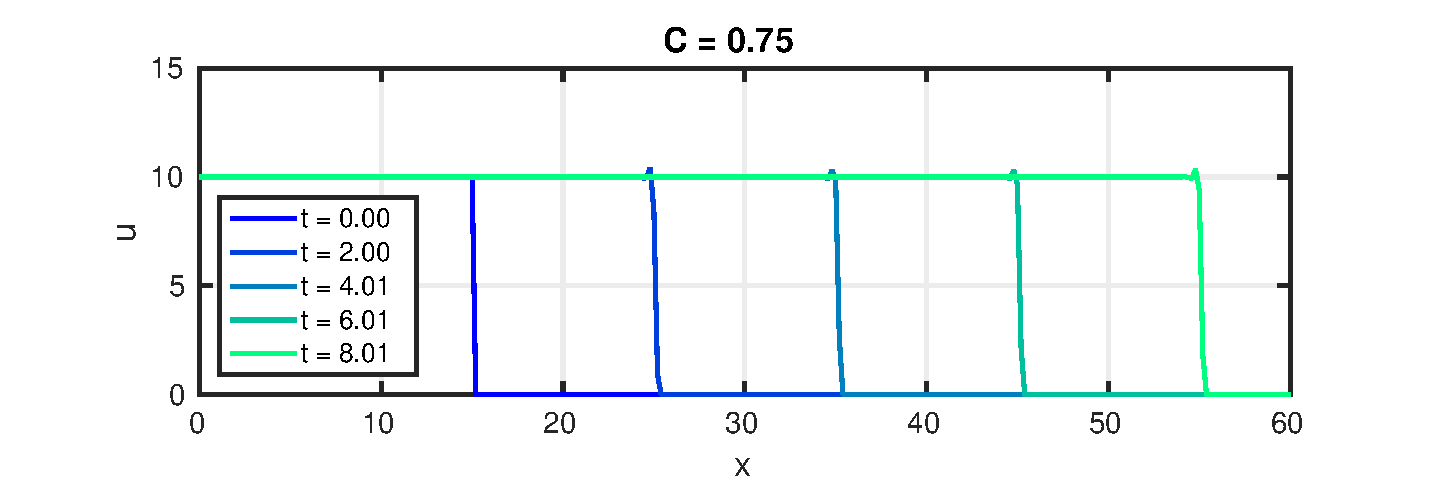
\includegraphics[width=0.85\textwidth]{Prob1_C075.eps} \\
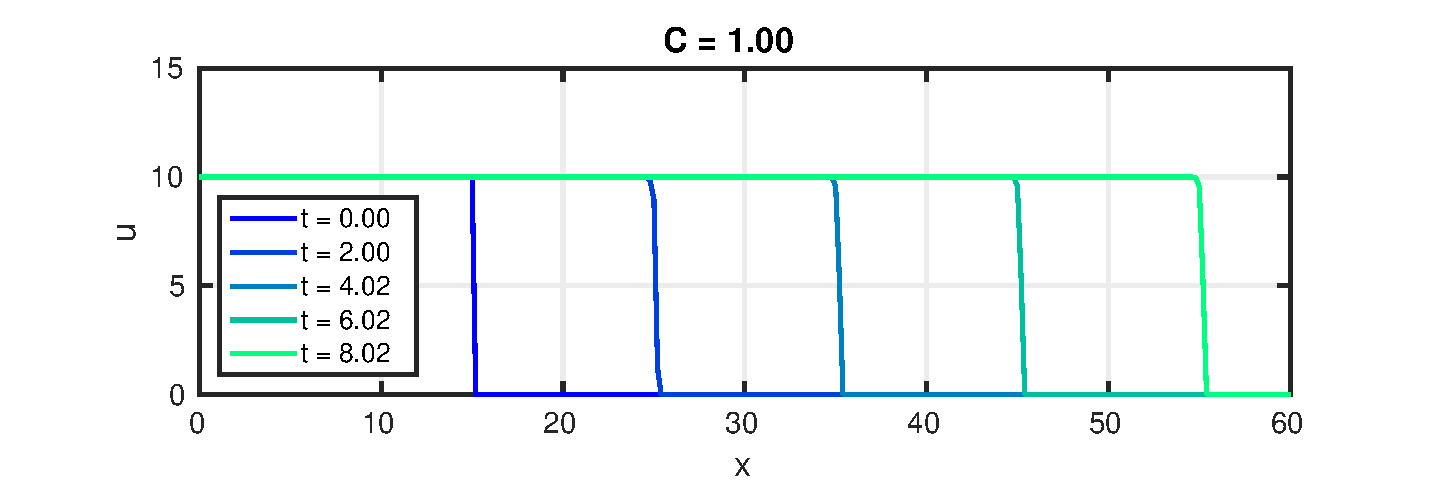
\includegraphics[width=0.85\textwidth]{Prob1_C100.eps} \\
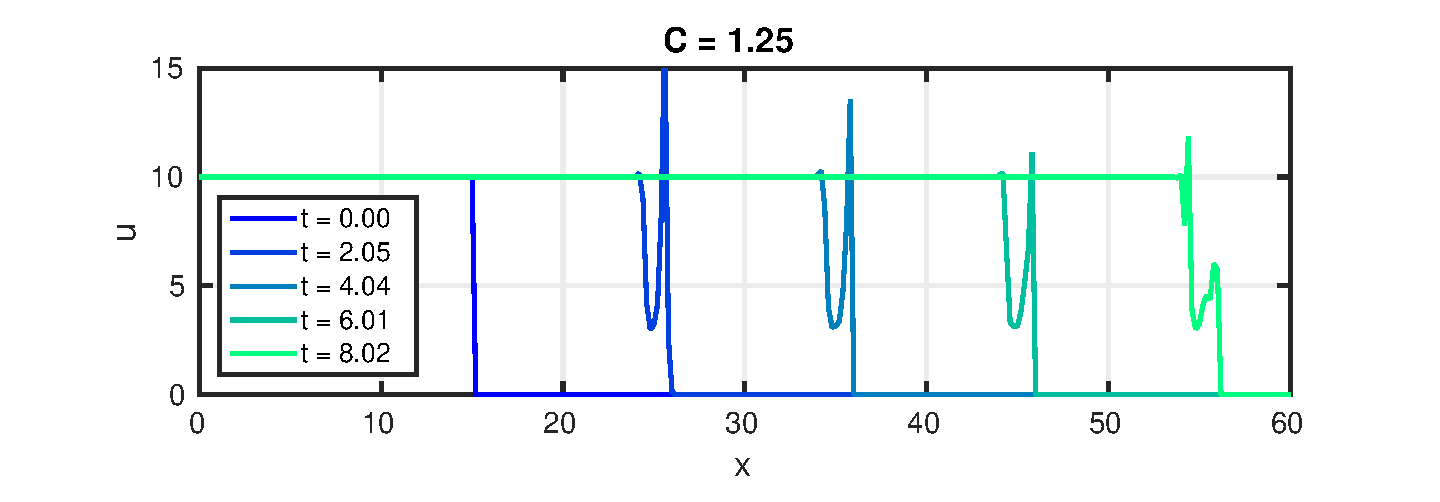
\includegraphics[width=0.85\textwidth]{Prob1_C125.eps} \\
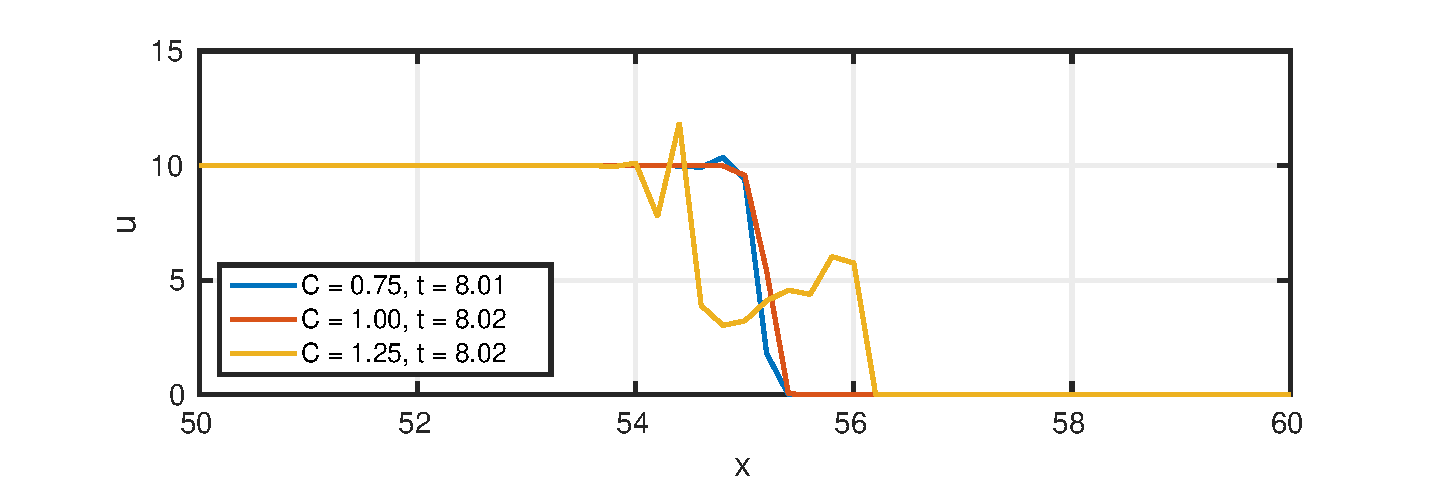
\includegraphics[width=0.85\textwidth]{Prob1_t8.eps}
\\[0.5cm]
\caption{MacCormack method solution for different Courant numbers, and comparison at time $t \sim 8$. The Courant number is seen to substantially affect the accuracy of the results.}
\label{fig:MacCormack}
\end{center}
\end{figure}

\begin{figure}[h!]
\begin{center}
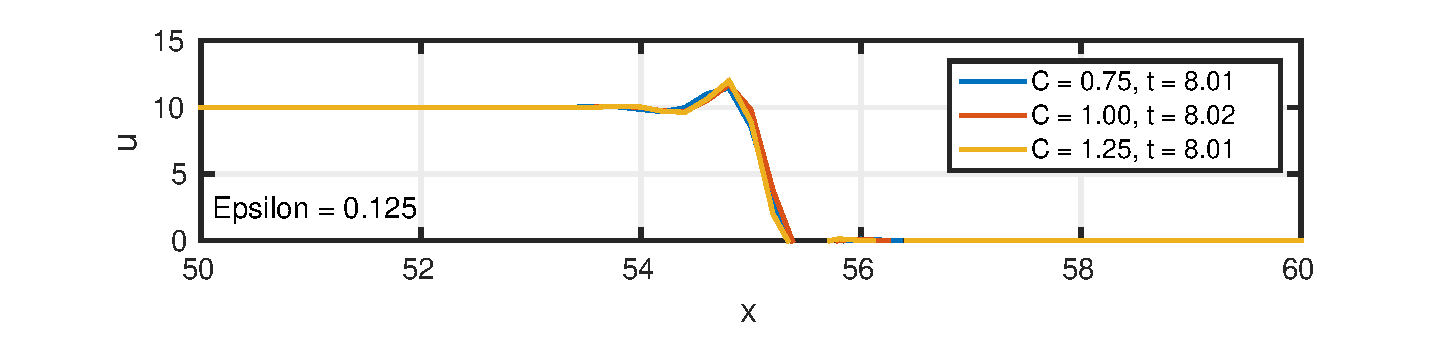
\includegraphics[width=0.85\textwidth]{Prob2_eps0125.eps} \vspace*{-0.5cm} \\
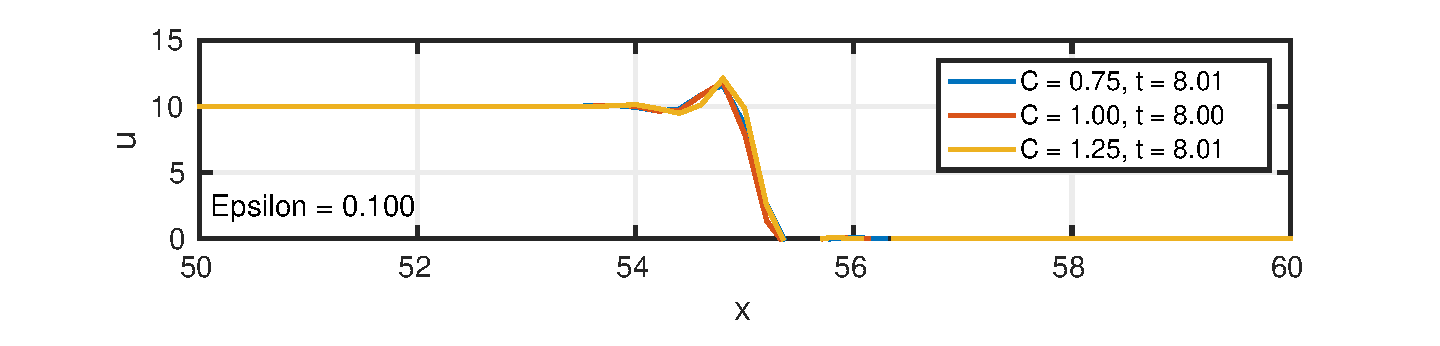
\includegraphics[width=0.85\textwidth]{Prob2_eps0100.eps} \vspace*{-0.5cm} \\
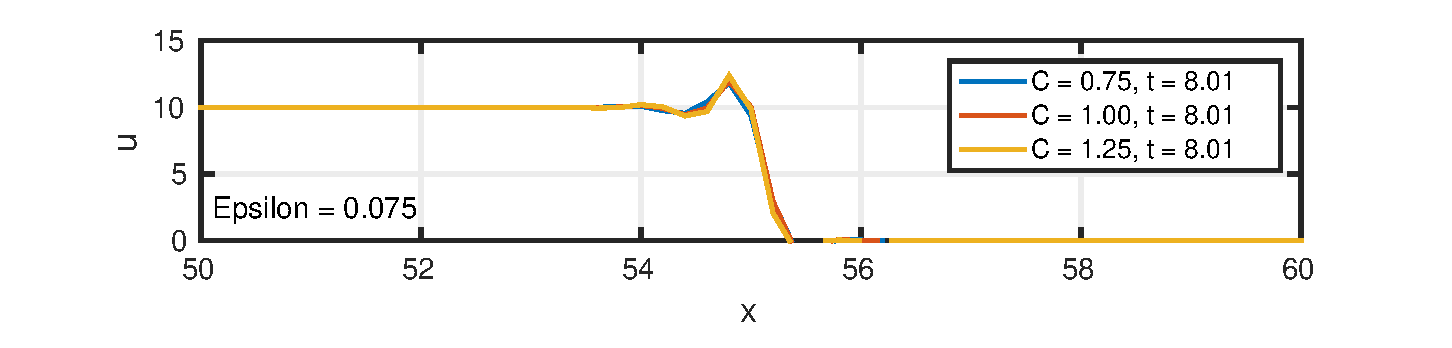
\includegraphics[width=0.85\textwidth]{Prob2_eps0075.eps} \vspace*{-0.5cm} \\
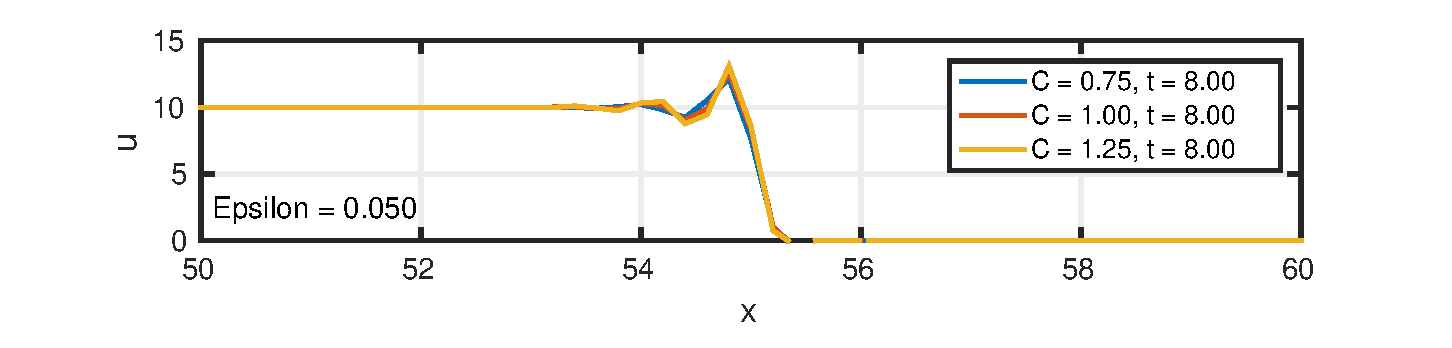
\includegraphics[width=0.85\textwidth]{Prob2_eps0050.eps} \vspace*{-0.5cm} \\
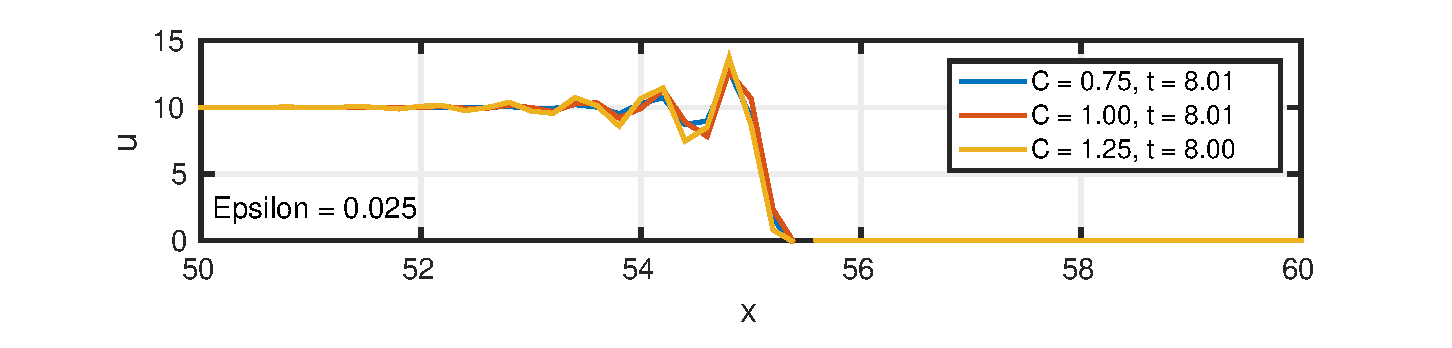
\includegraphics[width=0.85\textwidth]{Prob2_eps0025.eps} \vspace*{-0.5cm} \\
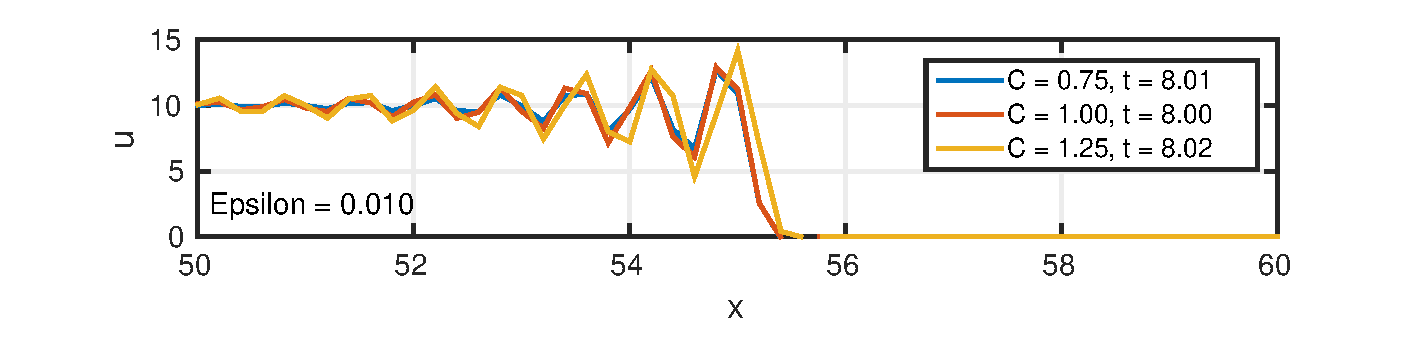
\includegraphics[width=0.85\textwidth]{Prob2_eps0010.eps} \vspace*{-0.5cm} \\
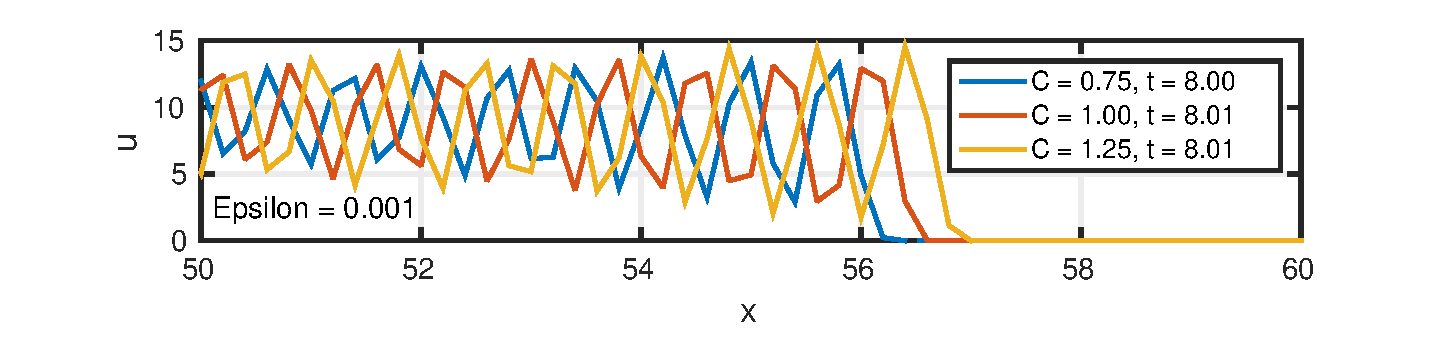
\includegraphics[width=0.85\textwidth]{Prob2_eps0001.eps}
\\[0.5cm]
\caption{Beam and Warming solution for different values of the dissipation term's coefficient $\epsilon$. Solutions at time $t \sim 8$ are shown for different Courant numbers in each plot. The solution diverged for values of $\epsilon$ even a few percent above 0.125. A value of $\epsilon=0.1$ appears to be sufficient.}
\label{fig:BeamWarming_Epsilon}
\end{center}
\end{figure}

\begin{figure}[h!]
\begin{center}
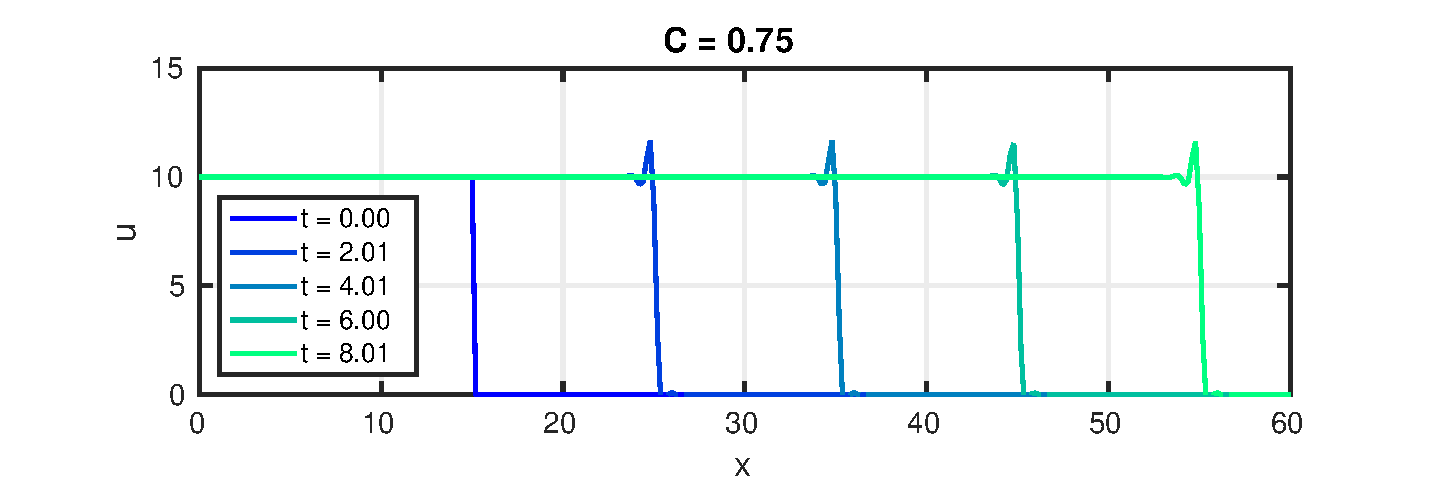
\includegraphics[width=0.85\textwidth]{Prob2_C075.eps} \\
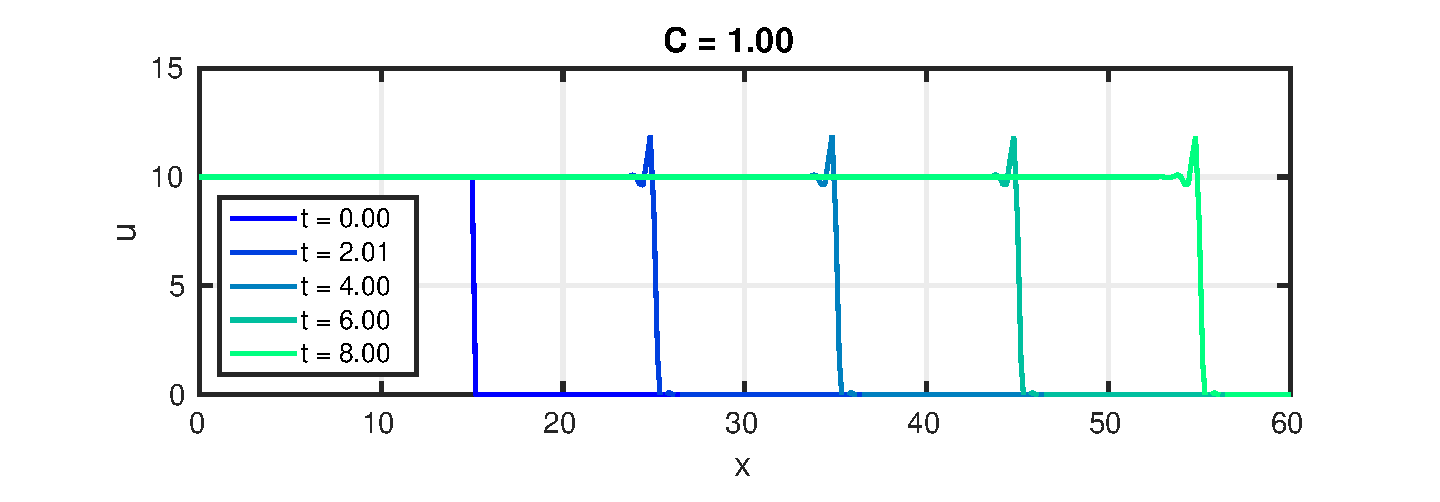
\includegraphics[width=0.85\textwidth]{Prob2_C100.eps} \\
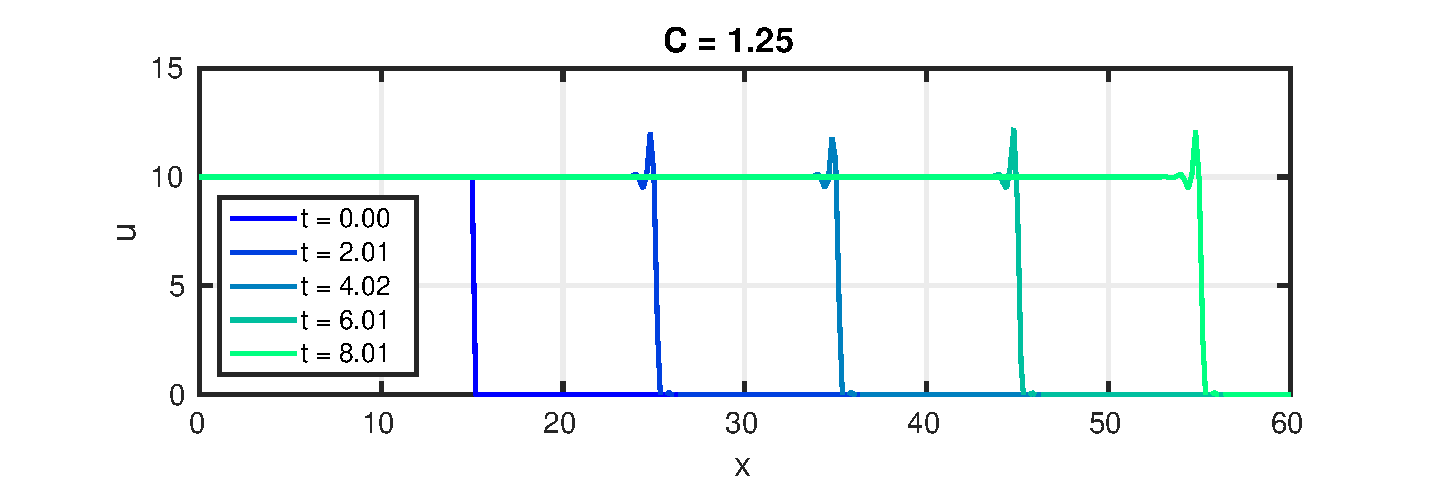
\includegraphics[width=0.85\textwidth]{Prob2_C125.eps} \\
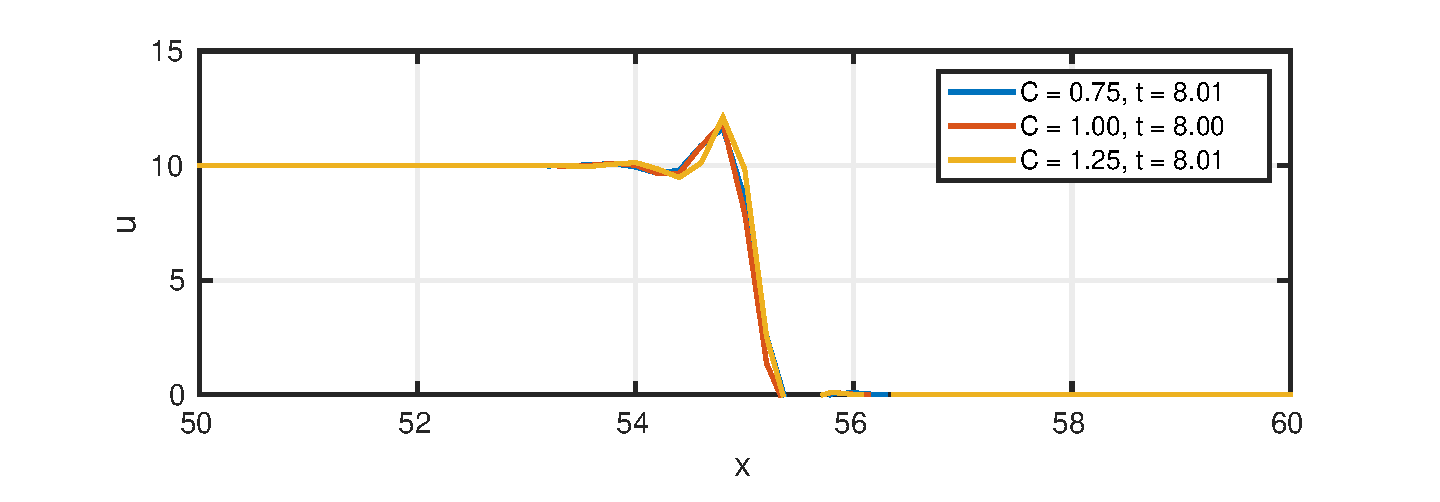
\includegraphics[width=0.85\textwidth]{Prob2_t8.eps}
\\[0.5cm]
\caption{Beam and Warming method solution for three Courant numbers, and comparison at time $t \sim 8$. The dissipation coefficient is $\epsilon = 0.1$. Little difference is observed between different Courant numbers.}
\label{fig:MacCormack}
\end{center}
\end{figure}

%%%%%%%%%%%%%%%%%%%%%%%%%%%%%%%%%%%%%%%%%%%%%%%%%
%%%%%%%%%%%%%%%%%%%%%%%%%%%%%%%%%%%%%%%%%%%%%%%%%
\section{Discussion} %%%%%%%%%%%%%%%%%%%%%%%%%%%%
%%%%%%%%%%%%%%%%%%%%%%%%%%%%%%%%%%%%%%%%%%%%%%%%%
%%%%%%%%%%%%%%%%%%%%%%%%%%%%%%%%%%%%%%%%%%%%%%%%%

%%%%%%%%%%%%%%%%%%%%%%%%%%%%%%%%%%%%%%%%%%%%%%%%%
%%%%%%%%%%%%%%%%%%%%%%%%%%%%%%%%%%%%%%%%%%%%%%%%%
\section{References} %%%%%%%%%%%%%%%%%%%%%%%%%%%%
%%%%%%%%%%%%%%%%%%%%%%%%%%%%%%%%%%%%%%%%%%%%%%%%%
%%%%%%%%%%%%%%%%%%%%%%%%%%%%%%%%%%%%%%%%%%%%%%%%%

No external references were used other than the course notes for this assignment.

%%%%%%%%%%%%%%%%%%%%%%%%%%%%%%%%%%%%%%%%%%%%%%%%%
%%%%%%%%%%%%%%%%%%%%%%%%%%%%%%%%%%%%%%%%%%%%%%%%%
\section*{Appendix: MATLAB Code} %%%%%%%%%%%%%%%%
%%%%%%%%%%%%%%%%%%%%%%%%%%%%%%%%%%%%%%%%%%%%%%%%%
%%%%%%%%%%%%%%%%%%%%%%%%%%%%%%%%%%%%%%%%%%%%%%%%%

The following code listings generate all figures presented in this homework assignment.

%\includecode{Problem_1.m}

%%
%% DOCUMENT END
%%
\end{document}
